%%%%%%%%%%%%%%%%%%%%%%%%%% lecture-2
%\begin{frame}
%  \frametitle{lecture-2 算法---程序的灵魂}
%  \tableofcontents[hideallsubsections]
%\end{frame}

\section{开发工具}

\begin{frame}{运行C程序的步骤与方法}
\centering
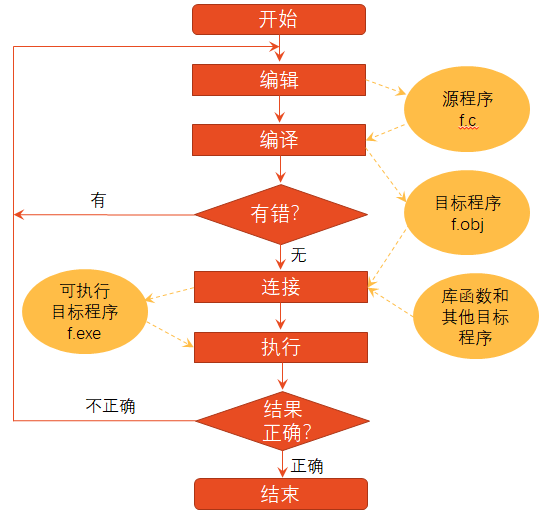
\includegraphics[scale=0.45]{program4}
\end{frame}

\begin{frame}{集成开发环境---编译系统}
\begin{itemize}
\setlength{\itemsep}{.5cm}
\item Bloodshed Dev-C++ 
\item Turbo C
\item Visual C++6.0 
\item Visual Studio(VS2015,VS Community 2019等)
\end{itemize}
\end{frame}

\begin{frame}{Bloodshed Dev-C++集成开发环境}
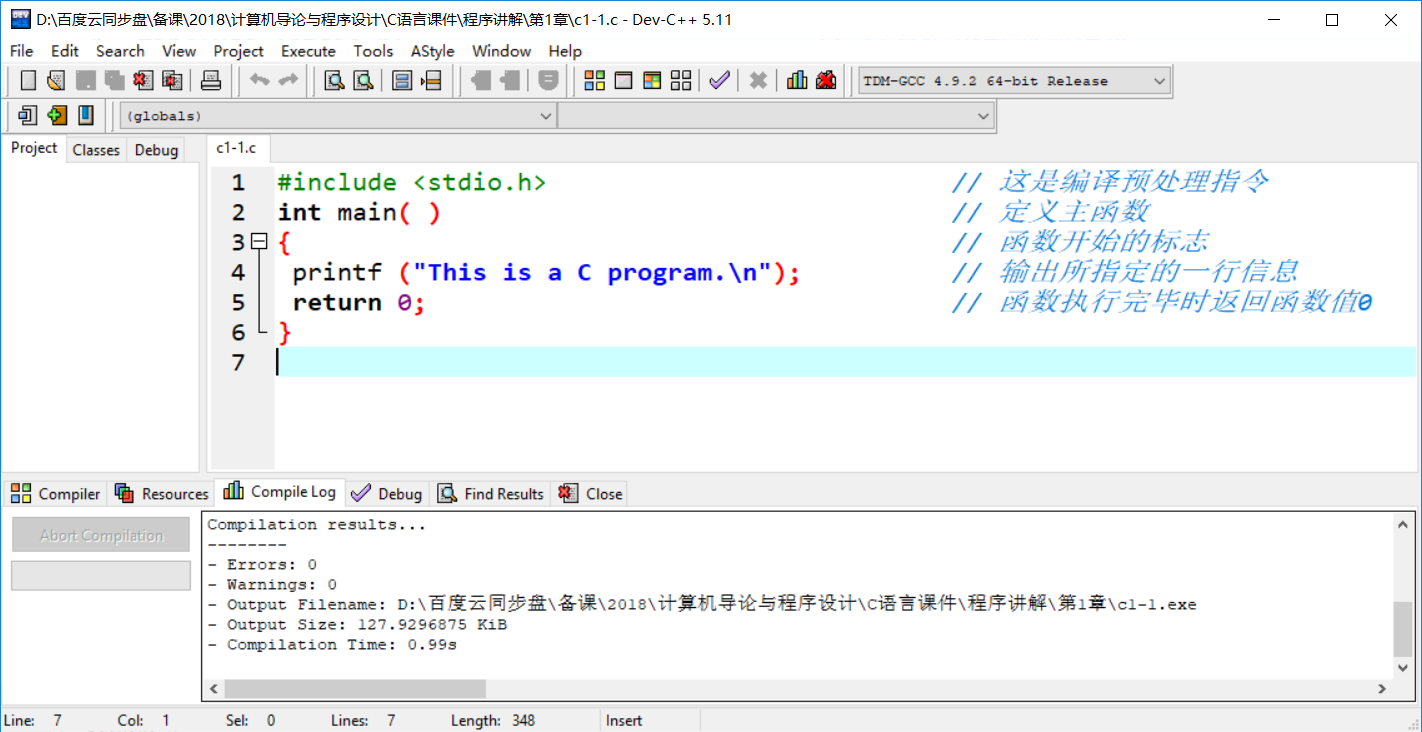
\includegraphics[scale=0.24]{DevCpp}   
\end{frame}

\begin{frame}{Bloodshed Dev-C++集成开发环境}
\begin{itemize}
\item 选择“文件”菜单,选择“源文件”, 编辑程序。
\item 保存时,保存为 .cpp或 .c文件。
\item 选择“编译和运行”菜单,生成.exe文件,运行程序。  
\end{itemize}
\centering 
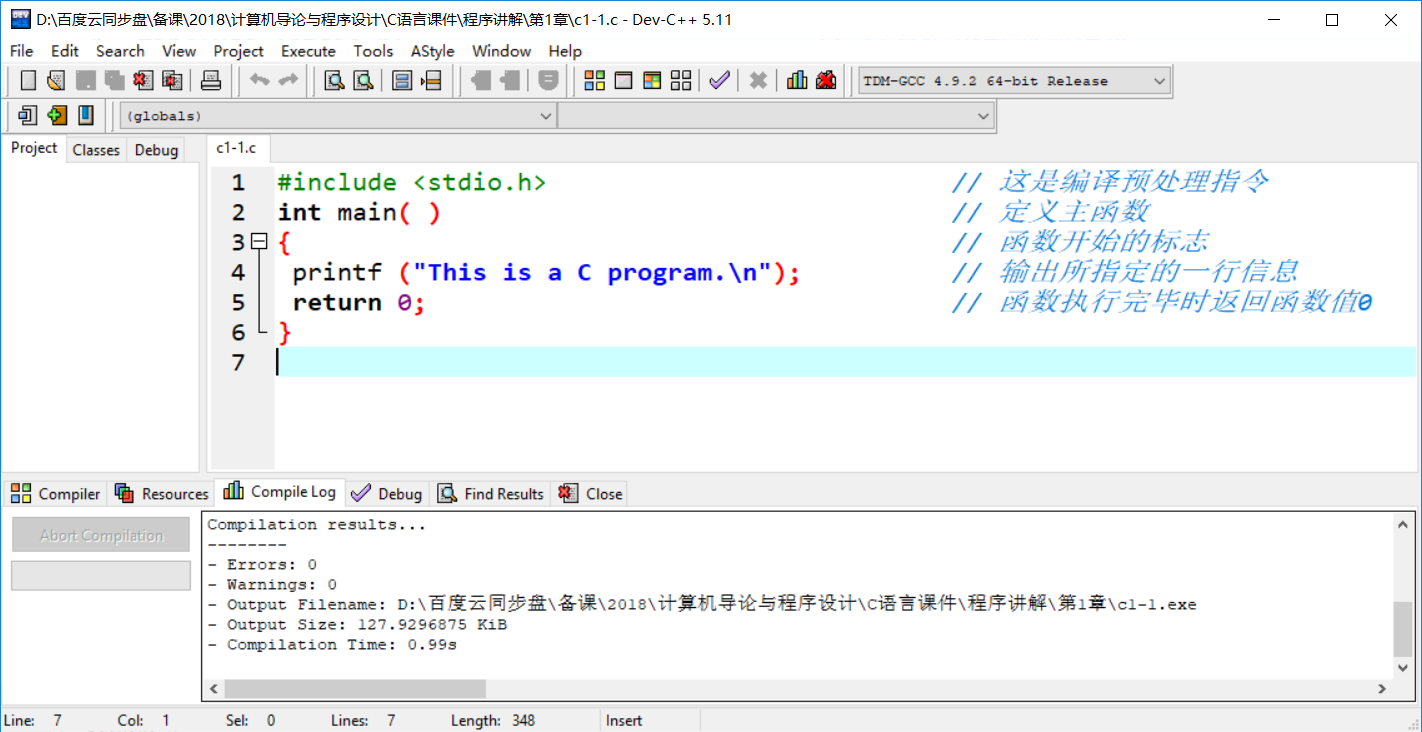
\includegraphics[scale=0.2]{DevCpp}   
\end{frame}

\section{Algorithm + Data Structures = Programs}

\begin{frame}{数据结构与算法}
\begin{columns}
	\column{0.4\textwidth}
	\begin{block}{}
		算法 + 数据结构 = 程序\\
		Algorithm + Data Structures = Programs
	\end{block}
    %\hspace{20pt}
	\column{0.4\textwidth}
	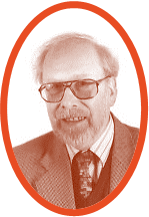
\includegraphics[scale=0.4]{Wirth}\\
	沃思(Niklaus Wirth)
\end{columns}
\begin{itemize}
	\item 数据结构\\
	对数据的描述。在程序中要指定用到哪些数据,以及这些数据的类型和数据的组织形式。
	\item 	算法\\
	对操作的描述。即要求计算机进行操作的步骤	
\end{itemize}
\end{frame}

\begin{frame}{程序员的工作}
\centering
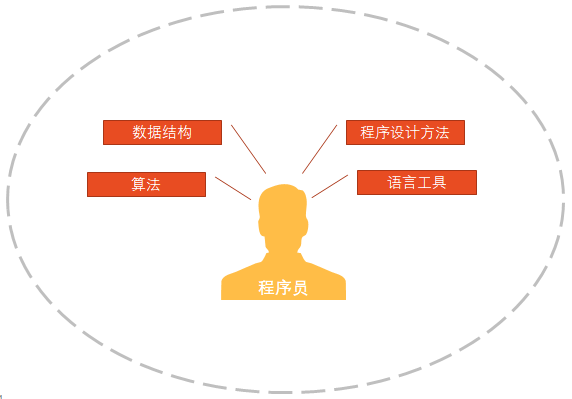
\includegraphics[scale=0.5]{programer}
\end{frame}

\begin{frame}{算法}
\begin{columns}
	\column{0.4\textwidth}
	
\includegraphics[scale=0.25]{programer2}
	\column{0.5\textwidth}
	\begin{block}{算法}
		\begin{itemize}
			\item 广义地说,为解决一个问题而采取的方法和步骤,就称为“算法”。
		    \item 对同一个问题,可以有不同的解题方法和步骤。
		    \item 为了有效地进行解题,不仅需要保证算法正确,还要考虑算法的质量,选择合适的算法。
		\end{itemize} 
	\end{block}
\end{columns}
\end{frame}

\begin{frame}{算法}
\begin{columns}[t]
	\column{0.45\textwidth}
	\begin{block}{数值运算算法}
	   如求一个方程的根, 计算一个函数的定积分等。\\
	   数值运算的目的是求数值解。\\
	   由于数值运算往往有现成的模型,可以运用数值分析方法,因此对数值运算的算法的研究比较深入,算法比较成熟。	
	\end{block}
	\column{0.45\textwidth}
	\begin{block}{非数值运算算法}
		如图书检索, 人事管理等。\\
		计算机在非数值运算方面的应用远超在数值运算方面的应用。
		非数值运算的种类繁多,要求各异,需要使用者参考已有的类似算法,重新设计解决特定问题的专门算法。
	\end{block}
\end{columns}
\end{frame}

\begin{frame}[shrink]{简单的算法举例[例2.1(p17)]}
\begin{example}
	[例2.1(p17)] 求$1\times 2\times 3\times 4\times 5$
\end{example}
\vspace{-0.7cm}
\small
\begin{columns}[t]
	\column{0.45\textwidth}
	\begin{block}{算法(一)步骤}<1->
		\begin{enumerate}
			\item[S1] 先求1乘以2,得到结果2
			\item[S2] 将步骤1得到的乘积2再乘以3,得到结果6
			\item[S3] 将6再乘以4,得24
			\item[S4] 将24再乘以5,得120
		\end{enumerate}	
	\end{block}
    \begin{block}{思考}<3->
    	求$1\times 3\times 5\times 7\times 9$
    \end{block}
	\column{0.45\textwidth}<2->
	\begin{block}{算法(二)步骤}
		\begin{enumerate}
			\item[S1] $p=1$, 表示将1存放在变量p中
			\item[S2] $i=2$, 表示将2存放在变量i中
			\item[S3] $p=p*i$, 使p与i相乘,乘积仍放在变量p中
			\item[S4] $i=i+1$, 使变量i的值加1
			\item[S5] if (i<=5) goto S3\\
			          else 算法结束, 最后得到p的值就是5!的值。
		\end{enumerate}	
	\end{block}
\end{columns}
\end{frame}

\begin{frame}[shrink]{简单的算法举例[例2.2(p18)]}
\begin{example}
	[例2.2(p18)] 有50个学生,要求输出成绩在80分以上的学生的学号和成绩.
\end{example}

\begin{block}{算法步骤}<2->
	float g[50]=\{100,90.5,30.8,$\cdots$\}; \textcolor{red}{// 表示50名学生成绩}\\
	int i = 0;  \textcolor{red}{//表示第i个学生学号}\\
	while(i<50) \\
	\{ \\
	   \qquad if (g[i]>=80) printf("第\%d个学生成绩\%f, " , i+1, g[i]); \\
	   \qquad i = i + 1;\\
	\} 
\end{block}
\end{frame}

\begin{frame}{例2.3(p18): 闰年判定条件.}
\centering
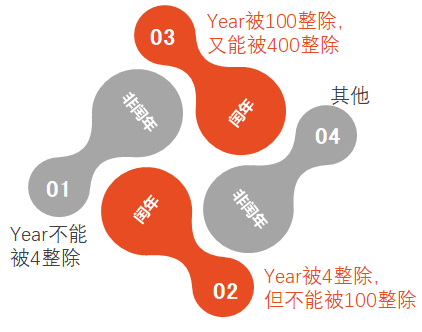
\includegraphics[scale=0.4]{leap}
\end{frame}

\note{
	1、普通闰年bai:公历年份是4的倍数的,一般是闰年。du(zhi如2004年就是闰年);
	
	2、世纪dao闰年:公历年份是整百数的,必须是400的倍数才是闰年(如1900年不是世纪闰年,2000年是世纪闰年)。
}

\begin{frame}[shrink]
\begin{columns}%[T] % align columns
	\begin{column}{1.0\textwidth}
		\begin{algorithm}[H]  
			\caption{例2.3(p18): 判定2000—2500年中的每一年是否为闰年.} %算法的名字
			\begin{algorithmic}[1] %每行显示行号
				\State int year=2000, char R; \textcolor{red}{// R是标志变量, 'Y'或'N'}
				\While{(year<=2500)} % While语句,需要和EndWhile对应
				\State R=`N';  
				\If{(year能被4整除,但是不能被100整除)} R=`Y'; % If 语句,需要和EndIf对应
				\ElsIf {(year能被100整除, 并且能被400整除)} R=`Y';
				\EndIf
				\If{(R=='Y')} printf(``\%d是闰年", year); 
				\Else \quad printf(``\%d不是闰年", year);
				\EndIf	
				\State year = year + 1;
				\EndWhile
			\end{algorithmic}  
		\end{algorithm}
	\end{column}%
\end{columns}

%%%%%%%%%%%%% 会引起目录页有此图
%\begin{textblock*}{15cm}(8.5cm,5cm)
%	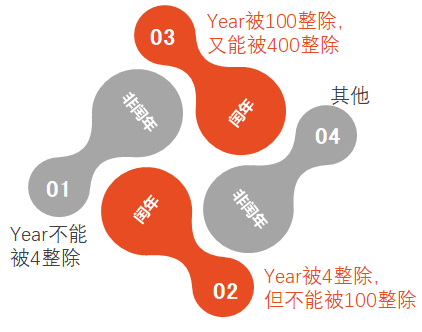
\includegraphics[scale=0.25]{leap}
%\end{textblock*}
\end{frame}

\begin{frame}%[shrink]
\begin{columns}%[T] % align columns
	\begin{column}<0->{.8\textwidth}
		%\scriptsize
		\begin{algorithm}[H]  
			\caption{例2.4(p19): 求$1-\frac{1}{2}+\frac{1}{3}-\frac{1}{4}+\cdots+\frac{1}{99}-\frac{1}{100}$.} %算法的名字
			\begin{algorithmic}[1] %每行显示行号
				\State int sign=1, deno=2;
				\State float sum = 1.0; 
				\While{(deno<=100)} % While语句,需要和EndWhile对应
				\State sign = -1 * sign;
				\State sum = sum + sign*1.0/deno; 
				\State deno = deno + 1; 
				\EndWhile
				\State printf(``sum=\%f$\backslash$n", sum);	
			\end{algorithmic}  
		\end{algorithm}
	\end{column}%
	%\hfill%	
	\begin{column}<0->{.20\textwidth}
		\newline
		\newline
		sign: 表示当前项的数值符号\\
		deno: 表示当前项的分母\\
		sum:  表示当前项的累加和
	\end{column}%
\end{columns}
\medskip
\colorbox{green}{问题: 为何使用sign*1.0 ?}
\end{frame}

\begin{frame}%[shrink]
\begin{columns}%[T] % align columns
	\begin{column}<0->{1.0\textwidth}
		%\scriptsize
		\begin{algorithm}[H]  
			\caption{例2.5(p20): 给出一个大于或等于3的正整数,判断它是不是一个素数.} %算法的名字
			\begin{algorithmic}[1] %每行显示行号
				\State int n, i=2;
				\State scanf("\%d",\&n); \textcolor{red}{// 输入n的值.} 
				\While{(i < n)} % While语句,需要和EndWhile对应
				\If{(n能被i整除)} \{ printf(``\%d不是素数", n); return; \}
				\EndIf
				\State i = i + 1;
				\EndWhile
				\State printf(``\%d是素数", n);	
			\end{algorithmic}  
		\end{algorithm}
	\end{column}%
	%\hfill%	
\end{columns}
\begin{block}{Notes}
	实际上, $n$不必检查被$2\sim(n-1)$之间的整数整除, 只须检查能否被$2\sim\sqrt{2}$间的整数整除即可。
\end{block}
\end{frame}

\begin{frame}{算法的特性}
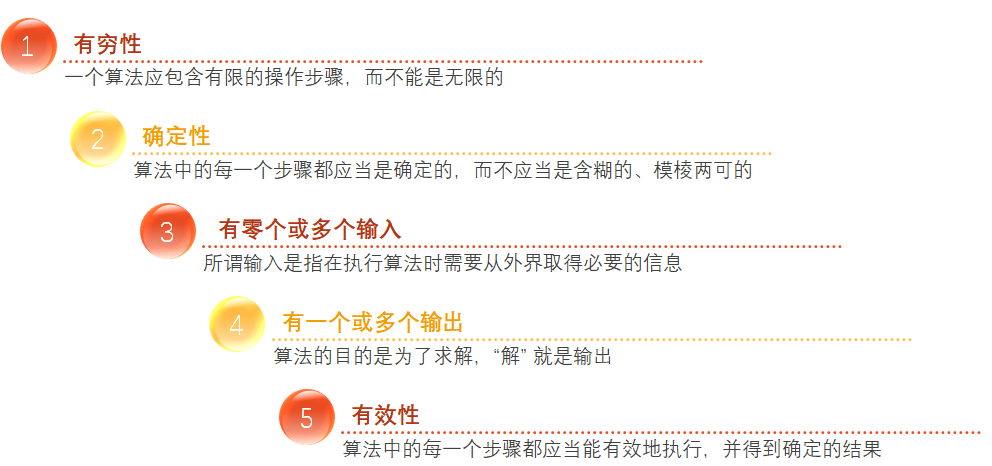
\includegraphics[scale=0.35]{algo}
\end{frame}

\begin{frame}{结构化程序设计方法}
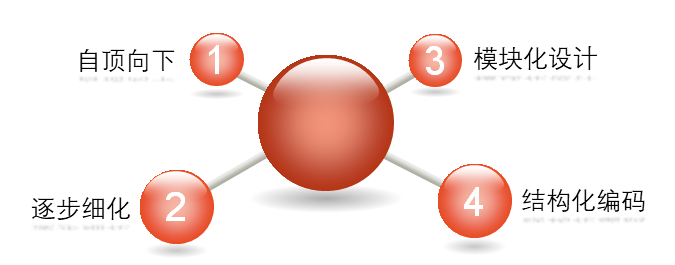
\includegraphics[scale=0.5]{top-down}
\end{frame}

\section{初识C语言程序}

\begin{frame}[fragile]{求5!的C语言程序。\small{[作业: 请抄写以下各页,并试着分析理解。]}}
\begin{lstlisting}
#include<stdio.h>            // standard input/output编译预处理指令
int main()                   // 主函数
{                            // 函数开始标志
   int i,p;  // p表示被乘数, i表示乘数
   p=1;
   i=2;
   while(i<=5)
   {  
      p=p*i;
      i++; // i = i + 1
   }
   printf("%d\n",p);
   return 0;                 // 函数执行完毕返回函数值0
}                            // 函数结束标志
\end{lstlisting}
\end{frame}

\begin{frame}[fragile]{变量在使用之前首先要定义它的数据类型}
\begin{lstlisting}
#include<stdio.h>            // standard input/output编译预处理指令
int main()                   // 主函数
{                            // 函数开始标志
   int a,b;  // 定义变量a, b为整型数值,同类型变量可以在一条语句中定义。
   float f;  // 定义变量f为单精度浮点数
   double d; // 定义变量d为双精度浮点数
   char c;   // 定义变量c为单个英文字母
   a=10;
   b=20;
   f=10.2;
   d=20.3;
   c='A';
   return 0;                 // 函数执行完毕返回函数值0
}                            // 函数结束标志
\end{lstlisting}
\end{frame}

\begin{frame}{常用格式描述符与数据类型的对应关系}
\begin{tabular}{|c|c|c|}
	\hline 
	\textbf{格式符} & \textbf{对应的数据类型} &  \textbf{备注}\\ 
	\hline 
	\%d & int &  \\ 
	\hline  
	\%f & float &  \\
	\hline
	\%c & char & \\ 
	\hline   
	\%lf & double & \\ 
	\hline 
	\%.2f & float & 保留两位小数, 四舍五入。不适用于scanf()。 \\ 
	\hline 
	\%.2lf & double & 保留两位小数, 四舍五入。不适用于scanf()。 \\ 
	\hline
	\hline   
	\%x & int & 十六进制显示 \\ 
	\hline 
	\%ld & long int &  \\ 
	\hline 
\end{tabular}
\newline
\newline
\textcolor{blue}{详见p73, 表3.6}
\end{frame}

\begin{frame}[fragile]{输出语句printf(``原样输出, \%格式符'', 对应变量值);}
\begin{lstlisting}
#include<stdio.h>            // standard input/output编译预处理指令
int main()                   // 主函数
{                            // 函数开始标志
   int a=10,b;    // 定义变量a, b为整型数值, 定义变量时,可以指定变量的初值
   float f=10.2;  // 定义变量f为单精度浮点数
   double d; // 定义变量d为双精度浮点数
   char c;   // 定义变量c为单个英文字母
   f=10.2;
   d=20.3;
   c='A';
   printf("a=%d,b=%d,c=%c,f=%f,d=%lf\n",a,b,c,f,d); // \n为换行符
   return 0;                 // 函数执行完毕返回函数值0
}                            // 函数结束标志
\end{lstlisting}
\end{frame}

\begin{frame}[fragile]{输入语句scanf(``\%变量格式符'', \&变量名);}
\begin{lstlisting}
#include<stdio.h>            // standard input/output编译预处理指令
int main()                   // 主函数
{                            // 函数开始标志
    int a=10,b;    // 定义变量a, b为整型数值, 定义变量时,可以指定变量的初值
    float f=10.2;  // 定义变量f为单精度浮点数
    double d; // 定义变量d为双精度浮点数
    char c='A';   // 定义变量c为单个英文字母, 字符输入以后讲
    printf("请输入整数a,b, 空格隔开:\n"); // 提示语句[可选]
    scanf("%d%d",&a,&b);
    printf("请输入浮点数f,d, 空格隔开:\n"); // 提示语句[可选]
    scanf("%f%lf",&f,&d);
    printf("a=%d,b=%d,c=%c,f=%f,d=%lf\n",a,b,c,f,d); // \n为换行符
    return 0;                 // 函数执行完毕返回函数值0
}                            // 函数结束标志
\end{lstlisting}
\end{frame}

\begin{frame}[fragile]{if(条件表达式)\{ 表达式为真(非0)时执行语句; \}}
\begin{lstlisting}
#include<stdio.h>            // standard input/output编译预处理指令
int main()                   // 主函数
{                            // 函数开始标志
   int a=10;    // 定义变量a为整型数值, 定义变量时,可以指定变量的初值
   if(a>=10)
   {
      printf("a>=10\n"); // \n为换行符
   }
   else
   {
      printf("a<10\n"); // \n为换行符
   }
   return 0;                 // 函数执行完毕返回函数值0
}                            // 函数结束标志
\end{lstlisting}
\end{frame}

\begin{frame}[fragile]{while(条件表达式)\{ 表达式为真(非0)时执行的语句;\}}
\begin{lstlisting}
#include<stdio.h>            // standard input/output编译预处理指令
int main()                   // 主函数
{                            // 函数开始标志
   int a=10;    // 定义变量a为整型数值, 定义变量时,可以指定变量的初值
   while(a>=0)
   {
     printf("a=%d\n",a); // \n为换行符
     a--; // a= a - 1
   }
   return 0;                 // 函数执行完毕返回函数值0
}                            // 函数结束标志
\end{lstlisting}
\end{frame}



